\documentclass[1p]{elsarticle_modified}
%\bibliographystyle{elsarticle-num}

%\usepackage[colorlinks]{hyperref}
%\usepackage{abbrmath_seonhwa} %\Abb, \Ascr, \Acal ,\Abf, \Afrak
\usepackage{amsfonts}
\usepackage{amssymb}
\usepackage{amsmath}
\usepackage{amsthm}
\usepackage{scalefnt}
\usepackage{amsbsy}
\usepackage{kotex}
\usepackage{caption}
\usepackage{subfig}
\usepackage{color}
\usepackage{graphicx}
\usepackage{xcolor} %% white, black, red, green, blue, cyan, magenta, yellow
\usepackage{float}
\usepackage{setspace}
\usepackage{hyperref}

\usepackage{tikz}
\usetikzlibrary{arrows}

\usepackage{multirow}
\usepackage{array} % fixed length table
\usepackage{hhline}

%%%%%%%%%%%%%%%%%%%%%
\makeatletter
\renewcommand*\env@matrix[1][\arraystretch]{%
	\edef\arraystretch{#1}%
	\hskip -\arraycolsep
	\let\@ifnextchar\new@ifnextchar
	\array{*\c@MaxMatrixCols c}}
\makeatother %https://tex.stackexchange.com/questions/14071/how-can-i-increase-the-line-spacing-in-a-matrix
%%%%%%%%%%%%%%%

\usepackage[normalem]{ulem}

\newcommand{\msout}[1]{\ifmmode\text{\sout{\ensuremath{#1}}}\else\sout{#1}\fi}
%SOURCE: \msout is \stkout macro in https://tex.stackexchange.com/questions/20609/strikeout-in-math-mode

\newcommand{\cancel}[1]{
	\ifmmode
	{\color{red}\msout{#1}}
	\else
	{\color{red}\sout{#1}}
	\fi
}

\newcommand{\add}[1]{
	{\color{blue}\uwave{#1}}
}

\newcommand{\replace}[2]{
	\ifmmode
	{\color{red}\msout{#1}}{\color{blue}\uwave{#2}}
	\else
	{\color{red}\sout{#1}}{\color{blue}\uwave{#2}}
	\fi
}

\newcommand{\Sol}{\mathcal{S}} %segment
\newcommand{\D}{D} %diagram
\newcommand{\A}{\mathcal{A}} %arc


%%%%%%%%%%%%%%%%%%%%%%%%%%%%%5 test

\def\sl{\operatorname{\textup{SL}}(2,\Cbb)}
\def\psl{\operatorname{\textup{PSL}}(2,\Cbb)}
\def\quan{\mkern 1mu \triangleright \mkern 1mu}

\theoremstyle{definition}
\newtheorem{thm}{Theorem}[section]
\newtheorem{prop}[thm]{Proposition}
\newtheorem{lem}[thm]{Lemma}
\newtheorem{ques}[thm]{Question}
\newtheorem{cor}[thm]{Corollary}
\newtheorem{defn}[thm]{Definition}
\newtheorem{exam}[thm]{Example}
\newtheorem{rmk}[thm]{Remark}
\newtheorem{alg}[thm]{Algorithm}

\newcommand{\I}{\sqrt{-1}}
\begin{document}

%\begin{frontmatter}
%
%\title{Boundary parabolic representations of knots up to 8 crossings}
%
%%% Group authors per affiliation:
%\author{Yunhi Cho} 
%\address{Department of Mathematics, University of Seoul, Seoul, Korea}
%\ead{yhcho@uos.ac.kr}
%
%
%\author{Seonhwa Kim} %\fnref{s_kim}}
%\address{Center for Geometry and Physics, Institute for Basic Science, Pohang, 37673, Korea}
%\ead{ryeona17@ibs.re.kr}
%
%\author{Hyuk Kim}
%\address{Department of Mathematical Sciences, Seoul National University, Seoul 08826, Korea}
%\ead{hyukkim@snu.ac.kr}
%
%\author{Seokbeom Yoon}
%\address{Department of Mathematical Sciences, Seoul National University, Seoul, 08826,  Korea}
%\ead{sbyoon15@snu.ac.kr}
%
%\begin{abstract}
%We find all boundary parabolic representation of knots up to 8 crossings.
%
%\end{abstract}
%\begin{keyword}
%    \MSC[2010] 57M25 
%\end{keyword}
%
%\end{frontmatter}

%\linenumbers
%\tableofcontents
%
\newcommand\colored[1]{\textcolor{white}{\rule[-0.35ex]{0.8em}{1.4ex}}\kern-0.8em\color{red} #1}%
%\newcommand\colored[1]{\textcolor{white}{ #1}\kern-2.17ex	\textcolor{white}{ #1}\kern-1.81ex	\textcolor{white}{ #1}\kern-2.15ex\color{red}#1	}

{\Large $\underline{12a_{0373}~(K12a_{0373})}$}

\setlength{\tabcolsep}{10pt}
\renewcommand{\arraystretch}{1.6}
\vspace{1cm}\begin{tabular}{m{100pt}>{\centering\arraybackslash}m{274pt}}
\multirow{5}{120pt}{
	\centering
	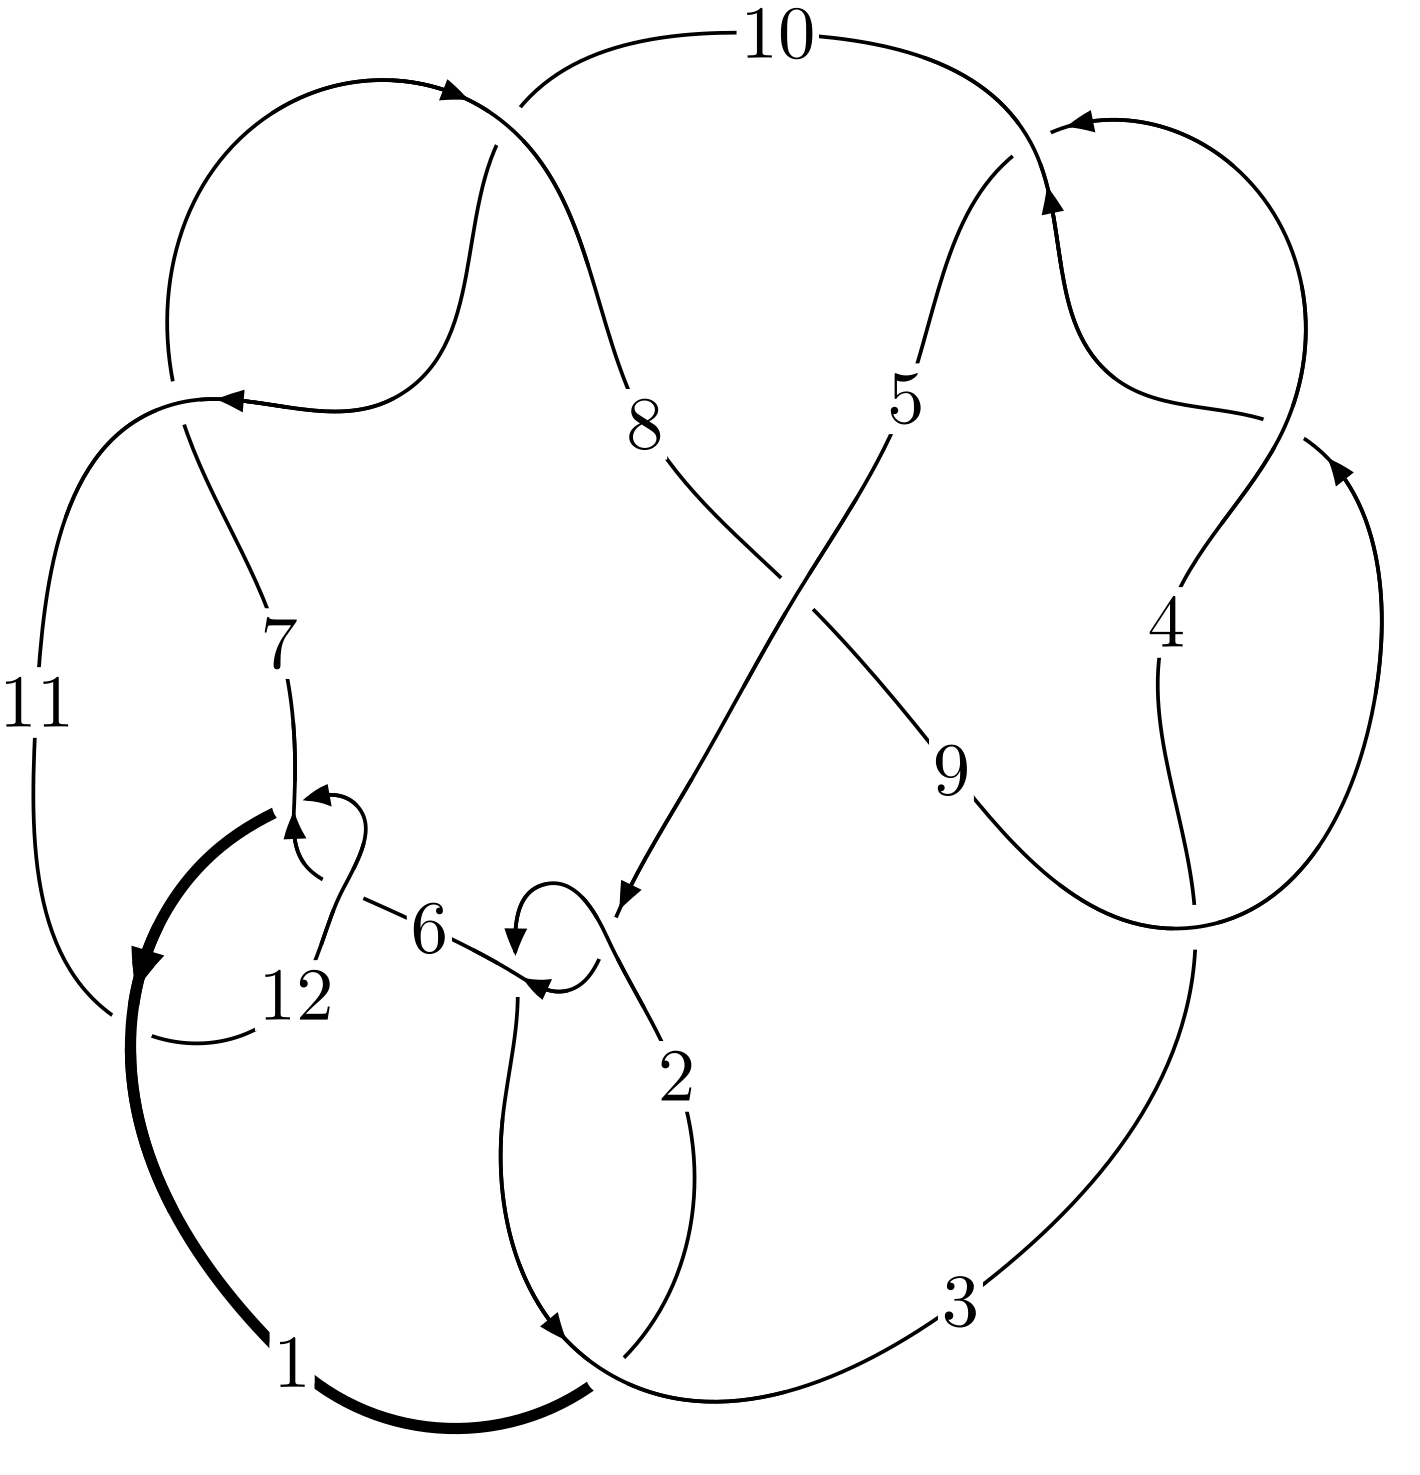
\includegraphics[width=112pt]{../../../GIT/diagram.site/Diagrams/png/1174_12a_0373.png}\\
\ \ \ A knot diagram\footnotemark}&
\allowdisplaybreaks
\textbf{Linearized knot diagam} \\
\cline{2-2}
 &
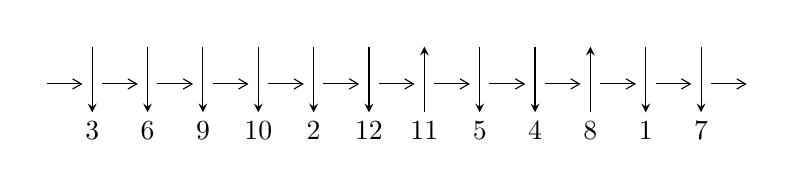
\begin{tikzpicture}[x=20pt, y=17pt]
	% nodes
	\node (C0) at (0, 0) {};
	\node (C1) at (1, 0) {};
	\node (C1U) at (1, +1) {};
	\node (C1D) at (1, -1) {3};

	\node (C2) at (2, 0) {};
	\node (C2U) at (2, +1) {};
	\node (C2D) at (2, -1) {6};

	\node (C3) at (3, 0) {};
	\node (C3U) at (3, +1) {};
	\node (C3D) at (3, -1) {9};

	\node (C4) at (4, 0) {};
	\node (C4U) at (4, +1) {};
	\node (C4D) at (4, -1) {10};

	\node (C5) at (5, 0) {};
	\node (C5U) at (5, +1) {};
	\node (C5D) at (5, -1) {2};

	\node (C6) at (6, 0) {};
	\node (C6U) at (6, +1) {};
	\node (C6D) at (6, -1) {12};

	\node (C7) at (7, 0) {};
	\node (C7U) at (7, +1) {};
	\node (C7D) at (7, -1) {11};

	\node (C8) at (8, 0) {};
	\node (C8U) at (8, +1) {};
	\node (C8D) at (8, -1) {5};

	\node (C9) at (9, 0) {};
	\node (C9U) at (9, +1) {};
	\node (C9D) at (9, -1) {4};

	\node (C10) at (10, 0) {};
	\node (C10U) at (10, +1) {};
	\node (C10D) at (10, -1) {8};

	\node (C11) at (11, 0) {};
	\node (C11U) at (11, +1) {};
	\node (C11D) at (11, -1) {1};

	\node (C12) at (12, 0) {};
	\node (C12U) at (12, +1) {};
	\node (C12D) at (12, -1) {7};
	\node (C13) at (13, 0) {};

	% arrows
	\draw[->,>={angle 60}]
	(C0) edge (C1) (C1) edge (C2) (C2) edge (C3) (C3) edge (C4) (C4) edge (C5) (C5) edge (C6) (C6) edge (C7) (C7) edge (C8) (C8) edge (C9) (C9) edge (C10) (C10) edge (C11) (C11) edge (C12) (C12) edge (C13) ;	\draw[->,>=stealth]
	(C1U) edge (C1D) (C2U) edge (C2D) (C3U) edge (C3D) (C4U) edge (C4D) (C5U) edge (C5D) (C6U) edge (C6D) (C7D) edge (C7U) (C8U) edge (C8D) (C9U) edge (C9D) (C10D) edge (C10U) (C11U) edge (C11D) (C12U) edge (C12D) ;
	\end{tikzpicture} \\
\hhline{~~} \\& 
\textbf{Solving Sequence} \\ \cline{2-2} 
 &
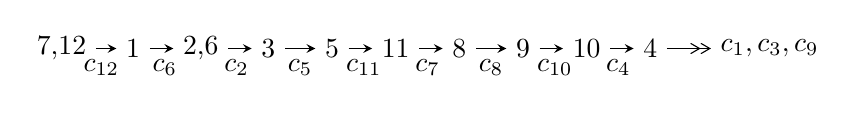
\begin{tikzpicture}[x=23pt, y=7pt]
	% node
	\node (A0) at (-1/8, 0) {7,12};
	\node (A1) at (1, 0) {1};
	\node (A2) at (33/16, 0) {2,6};
	\node (A3) at (25/8, 0) {3};
	\node (A4) at (33/8, 0) {5};
	\node (A5) at (41/8, 0) {11};
	\node (A6) at (49/8, 0) {8};
	\node (A7) at (57/8, 0) {9};
	\node (A8) at (65/8, 0) {10};
	\node (A9) at (73/8, 0) {4};
	\node (C1) at (1/2, -1) {$c_{12}$};
	\node (C2) at (3/2, -1) {$c_{6}$};
	\node (C3) at (21/8, -1) {$c_{2}$};
	\node (C4) at (29/8, -1) {$c_{5}$};
	\node (C5) at (37/8, -1) {$c_{11}$};
	\node (C6) at (45/8, -1) {$c_{7}$};
	\node (C7) at (53/8, -1) {$c_{8}$};
	\node (C8) at (61/8, -1) {$c_{10}$};
	\node (C9) at (69/8, -1) {$c_{4}$};
	\node (A10) at (11, 0) {$c_{1},c_{3},c_{9}$};

	% edge
	\draw[->,>=stealth]	
	(A0) edge (A1) (A1) edge (A2) (A2) edge (A3) (A3) edge (A4) (A4) edge (A5) (A5) edge (A6) (A6) edge (A7) (A7) edge (A8) (A8) edge (A9) ;
	\draw[->>,>={angle 60}]	
	(A9) edge (A10);
\end{tikzpicture} \\ 

\end{tabular} \\

\footnotetext{
The image of knot diagram is generated by the software ``\textbf{Draw programme}" developed by Andrew Bartholomew(\url{http://www.layer8.co.uk/maths/draw/index.htm\#Running-draw}), where we modified some parts for our purpose(\url{https://github.com/CATsTAILs/LinksPainter}).
}\phantom \\ \newline 
\centering \textbf{Ideals for irreducible components\footnotemark of $X_{\text{par}}$} 
 
\begin{align*}
I^u_{1}&=\langle 
- u^{26}+u^{25}+\cdots+2 b-1,\;- u^{26}+u^{25}+\cdots+2 a-3,\;u^{28}- u^{27}+\cdots+2 u-1\rangle \\
I^u_{2}&=\langle 
-319541245 u^{47}+177558344 u^{46}+\cdots+205886657 b+360357122,\\
\phantom{I^u_{2}}&\phantom{= \langle  }215527940 u^{47}+208732938 u^{46}+\cdots+205886657 a+1321032619,\;u^{48}- u^{47}+\cdots-8 u+1\rangle \\
I^u_{3}&=\langle 
b- a-1,\;a^2-2 a-1,\;u-1\rangle \\
I^u_{4}&=\langle 
b-2,\;a-1,\;u+1\rangle \\
\\
\end{align*}
\raggedright * 4 irreducible components of $\dim_{\mathbb{C}}=0$, with total 79 representations.\\
\footnotetext{All coefficients of polynomials are rational numbers. But the coefficients are sometimes approximated in decimal forms when there is not enough margin.}
\newpage
\renewcommand{\arraystretch}{1}
\centering \section*{I. $I^u_{1}= \langle - u^{26}+u^{25}+\cdots+2 b-1,\;- u^{26}+u^{25}+\cdots+2 a-3,\;u^{28}- u^{27}+\cdots+2 u-1 \rangle$}
\flushleft \textbf{(i) Arc colorings}\\
\begin{tabular}{m{7pt} m{180pt} m{7pt} m{180pt} }
\flushright $a_{7}=$&$\begin{pmatrix}0\\u\end{pmatrix}$ \\
\flushright $a_{12}=$&$\begin{pmatrix}1\\0\end{pmatrix}$ \\
\flushright $a_{1}=$&$\begin{pmatrix}1\\u^2\end{pmatrix}$ \\
\flushright $a_{2}=$&$\begin{pmatrix}\frac{1}{2} u^{26}-\frac{1}{2} u^{25}+\cdots- u+\frac{3}{2}\\\frac{1}{2} u^{26}-\frac{1}{2} u^{25}+\cdots- u+\frac{1}{2}\end{pmatrix}$ \\
\flushright $a_{6}=$&$\begin{pmatrix}u\\u\end{pmatrix}$ \\
\flushright $a_{3}=$&$\begin{pmatrix}\frac{1}{2} u^{26}-\frac{1}{2} u^{25}+\cdots- u+\frac{3}{2}\\\frac{1}{2} u^{26}-\frac{1}{2} u^{25}+\cdots- u+\frac{1}{2}\end{pmatrix}$ \\
\flushright $a_{5}=$&$\begin{pmatrix}\frac{1}{2} u^{27}-\frac{1}{2} u^{26}+\cdots- u^2+\frac{5}{2} u\\\frac{1}{2} u^{27}-\frac{1}{2} u^{26}+\cdots- u^2+\frac{3}{2} u\end{pmatrix}$ \\
\flushright $a_{11}=$&$\begin{pmatrix}- u^2+1\\- u^4\end{pmatrix}$ \\
\flushright $a_{8}=$&$\begin{pmatrix}u^5-2 u^3+u\\u^7- u^5+u\end{pmatrix}$ \\
\flushright $a_{9}=$&$\begin{pmatrix}-\frac{5}{2} u^{27}+3 u^{26}+\cdots-\frac{7}{2} u+\frac{1}{2}\\-2 u^{27}+\frac{5}{2} u^{26}+\cdots-3 u+\frac{1}{2}\end{pmatrix}$ \\
\flushright $a_{10}=$&$\begin{pmatrix}- u^8+3 u^6-3 u^4+1\\- u^{10}+2 u^8- u^6-2 u^4+u^2\end{pmatrix}$ \\
\flushright $a_{4}=$&$\begin{pmatrix}\frac{1}{2} u^{27}-\frac{1}{2} u^{26}+\cdots- u^2+\frac{7}{2} u\\u^{23}-5 u^{21}+\cdots+2 u^3+u\end{pmatrix}$\\&\end{tabular}
\flushleft \textbf{(ii) Obstruction class $= -1$}\\~\\
\flushleft \textbf{(iii) Cusp Shapes $= - u^{27}+u^{26}+8 u^{25}-7 u^{24}-34 u^{23}+26 u^{22}+91 u^{21}-62 u^{20}-163 u^{19}+106 u^{18}+183 u^{17}-128 u^{16}-92 u^{15}+100 u^{14}-68 u^{13}-20 u^{12}+154 u^{11}-51 u^{10}-107 u^9+67 u^8+10 u^7-26 u^6+29 u^5-2 u^4-19 u^3+14 u^2+5 u-16$}\\~\\
\newpage\renewcommand{\arraystretch}{1}
\flushleft \textbf{(iv) u-Polynomials at the component}\newline \\
\begin{tabular}{m{50pt}|m{274pt}}
Crossings & \hspace{64pt}u-Polynomials at each crossing \\
\hline $$\begin{aligned}c_{1},c_{11}\end{aligned}$$&$\begin{aligned}
&u^{28}+15 u^{27}+\cdots+8 u+1
\end{aligned}$\\
\hline $$\begin{aligned}c_{2},c_{5},c_{6}\\c_{12}\end{aligned}$$&$\begin{aligned}
&u^{28}+u^{27}+\cdots-2 u-1
\end{aligned}$\\
\hline $$\begin{aligned}c_{3},c_{4},c_{9}\end{aligned}$$&$\begin{aligned}
&u^{28}-3 u^{27}+\cdots-2 u-2
\end{aligned}$\\
\hline $$\begin{aligned}c_{7},c_{10}\end{aligned}$$&$\begin{aligned}
&u^{28}+3 u^{27}+\cdots-16 u-16
\end{aligned}$\\
\hline $$\begin{aligned}c_{8}\end{aligned}$$&$\begin{aligned}
&u^{28}+9 u^{27}+\cdots+162 u+38
\end{aligned}$\\
\hline
\end{tabular}\\~\\
\newpage\renewcommand{\arraystretch}{1}
\flushleft \textbf{(v) Riley Polynomials at the component}\newline \\
\begin{tabular}{m{50pt}|m{274pt}}
Crossings & \hspace{64pt}Riley Polynomials at each crossing \\
\hline $$\begin{aligned}c_{1},c_{11}\end{aligned}$$&$\begin{aligned}
&y^{28}+y^{27}+\cdots-16 y+1
\end{aligned}$\\
\hline $$\begin{aligned}c_{2},c_{5},c_{6}\\c_{12}\end{aligned}$$&$\begin{aligned}
&y^{28}-15 y^{27}+\cdots-8 y+1
\end{aligned}$\\
\hline $$\begin{aligned}c_{3},c_{4},c_{9}\end{aligned}$$&$\begin{aligned}
&y^{28}-27 y^{27}+\cdots-12 y+4
\end{aligned}$\\
\hline $$\begin{aligned}c_{7},c_{10}\end{aligned}$$&$\begin{aligned}
&y^{28}+25 y^{27}+\cdots-3840 y+256
\end{aligned}$\\
\hline $$\begin{aligned}c_{8}\end{aligned}$$&$\begin{aligned}
&y^{28}-15 y^{27}+\cdots-18188 y+1444
\end{aligned}$\\
\hline
\end{tabular}\\~\\
\newpage\flushleft \textbf{(vi) Complex Volumes and Cusp Shapes}
$$\begin{array}{c|c|c}  
\text{Solutions to }I^u_{1}& \I (\text{vol} + \sqrt{-1}CS) & \text{Cusp shape}\\
 \hline 
\begin{aligned}
u &= \phantom{-}0.921994 + 0.438316 I \\
a &= -0.76982 + 1.29038 I \\
b &= -1.76982 + 1.29038 I\end{aligned}
 & -1.75772 - 3.56547 I & -11.57837 + 4.88877 I \\ \hline\begin{aligned}
u &= \phantom{-}0.921994 - 0.438316 I \\
a &= -0.76982 - 1.29038 I \\
b &= -1.76982 - 1.29038 I\end{aligned}
 & -1.75772 + 3.56547 I & -11.57837 - 4.88877 I \\ \hline\begin{aligned}
u &= -0.980184 + 0.322710 I \\
a &= -1.17512 - 2.37431 I \\
b &= -2.17512 - 2.37431 I\end{aligned}
 & -8.48761 + 2.20286 I & -16.1598 - 6.7049 I \\ \hline\begin{aligned}
u &= -0.980184 - 0.322710 I \\
a &= -1.17512 + 2.37431 I \\
b &= -2.17512 + 2.37431 I\end{aligned}
 & -8.48761 - 2.20286 I & -16.1598 + 6.7049 I \\ \hline\begin{aligned}
u &= \phantom{-}0.774066 + 0.543182 I \\
a &= -0.135954 + 0.570759 I \\
b &= -1.135950 + 0.570759 I\end{aligned}
 & -1.36302 - 4.31651 I & -8.31039 + 7.39761 I \\ \hline\begin{aligned}
u &= \phantom{-}0.774066 - 0.543182 I \\
a &= -0.135954 - 0.570759 I \\
b &= -1.135950 - 0.570759 I\end{aligned}
 & -1.36302 + 4.31651 I & -8.31039 - 7.39761 I \\ \hline\begin{aligned}
u &= -0.990674 + 0.520560 I \\
a &= -1.20586 - 0.76603 I \\
b &= -2.20586 - 0.76603 I\end{aligned}
 & -0.24283 + 7.08786 I & -8.04162 - 9.83073 I \\ \hline\begin{aligned}
u &= -0.990674 - 0.520560 I \\
a &= -1.20586 + 0.76603 I \\
b &= -2.20586 + 0.76603 I\end{aligned}
 & -0.24283 - 7.08786 I & -8.04162 + 9.83073 I \\ \hline\begin{aligned}
u &= \phantom{-}0.078627 + 0.853313 I \\
a &= \phantom{-}0.876417 - 0.044224 I \\
b &= -0.1235830 - 0.0442237 I\end{aligned}
 & -7.82726 + 5.09468 I & -10.66054 - 2.85681 I \\ \hline\begin{aligned}
u &= \phantom{-}0.078627 - 0.853313 I \\
a &= \phantom{-}0.876417 + 0.044224 I \\
b &= -0.1235830 + 0.0442237 I\end{aligned}
 & -7.82726 - 5.09468 I & -10.66054 + 2.85681 I\\
 \hline 
 \end{array}$$\newpage$$\begin{array}{c|c|c}  
\text{Solutions to }I^u_{1}& \I (\text{vol} + \sqrt{-1}CS) & \text{Cusp shape}\\
 \hline 
\begin{aligned}
u &= \phantom{-}1.051900 + 0.542779 I \\
a &= -1.53095 + 0.56330 I \\
b &= -2.53095 + 0.56330 I\end{aligned}
 & -5.30353 - 10.40520 I & -13.0720 + 9.8966 I \\ \hline\begin{aligned}
u &= \phantom{-}1.051900 - 0.542779 I \\
a &= -1.53095 - 0.56330 I \\
b &= -2.53095 - 0.56330 I\end{aligned}
 & -5.30353 + 10.40520 I & -13.0720 - 9.8966 I \\ \hline\begin{aligned}
u &= -0.613429 + 0.514922 I \\
a &= \phantom{-}0.383789 - 0.430769 I \\
b &= -0.616211 - 0.430769 I\end{aligned}
 & \phantom{-}2.08348 + 1.42913 I & -1.76601 - 3.86378 I \\ \hline\begin{aligned}
u &= -0.613429 - 0.514922 I \\
a &= \phantom{-}0.383789 + 0.430769 I \\
b &= -0.616211 + 0.430769 I\end{aligned}
 & \phantom{-}2.08348 - 1.42913 I & -1.76601 + 3.86378 I \\ \hline\begin{aligned}
u &= -0.052810 + 0.786288 I \\
a &= \phantom{-}0.850234 + 0.019571 I \\
b &= -0.149766 + 0.019571 I\end{aligned}
 & -1.72551 - 1.99191 I & -6.96869 + 3.27675 I \\ \hline\begin{aligned}
u &= -0.052810 - 0.786288 I \\
a &= \phantom{-}0.850234 - 0.019571 I \\
b &= -0.149766 - 0.019571 I\end{aligned}
 & -1.72551 + 1.99191 I & -6.96869 - 3.27675 I \\ \hline\begin{aligned}
u &= -0.755899\phantom{ +0.000000I} \\
a &= \phantom{-}3.09480\phantom{ +0.000000I} \\
b &= \phantom{-}2.09480\phantom{ +0.000000I}\end{aligned}
 & -7.05303\phantom{ +0.000000I} & -9.54120\phantom{ +0.000000I} \\ \hline\begin{aligned}
u &= \phantom{-}0.439706 + 0.594385 I \\
a &= \phantom{-}0.593130 + 0.123123 I \\
b &= -0.406870 + 0.123123 I\end{aligned}
 & -1.78196 + 1.31248 I & -6.93906 - 0.09185 I \\ \hline\begin{aligned}
u &= \phantom{-}0.439706 - 0.594385 I \\
a &= \phantom{-}0.593130 - 0.123123 I \\
b &= -0.406870 - 0.123123 I\end{aligned}
 & -1.78196 - 1.31248 I & -6.93906 + 0.09185 I \\ \hline\begin{aligned}
u &= \phantom{-}1.222060 + 0.480272 I \\
a &= -2.62599 + 0.44865 I \\
b &= -3.62599 + 0.44865 I\end{aligned}
 & -8.88868 - 7.02526 I & -14.1377 + 3.4246 I\\
 \hline 
 \end{array}$$\newpage$$\begin{array}{c|c|c}  
\text{Solutions to }I^u_{1}& \I (\text{vol} + \sqrt{-1}CS) & \text{Cusp shape}\\
 \hline 
\begin{aligned}
u &= \phantom{-}1.222060 - 0.480272 I \\
a &= -2.62599 - 0.44865 I \\
b &= -3.62599 - 0.44865 I\end{aligned}
 & -8.88868 + 7.02526 I & -14.1377 - 3.4246 I \\ \hline\begin{aligned}
u &= -1.236550 + 0.456519 I \\
a &= -2.78618 - 0.51023 I \\
b &= -3.78618 - 0.51023 I\end{aligned}
 & -15.5795 + 3.9534 I & -17.7234 - 3.5115 I \\ \hline\begin{aligned}
u &= -1.236550 - 0.456519 I \\
a &= -2.78618 + 0.51023 I \\
b &= -3.78618 + 0.51023 I\end{aligned}
 & -15.5795 - 3.9534 I & -17.7234 + 3.5115 I \\ \hline\begin{aligned}
u &= -1.230830 + 0.503719 I \\
a &= -2.58655 - 0.30440 I \\
b &= -3.58655 - 0.30440 I\end{aligned}
 & -8.5405 + 11.5460 I & -13.2621 - 8.9561 I \\ \hline\begin{aligned}
u &= -1.230830 - 0.503719 I \\
a &= -2.58655 + 0.30440 I \\
b &= -3.58655 + 0.30440 I\end{aligned}
 & -8.5405 - 11.5460 I & -13.2621 + 8.9561 I \\ \hline\begin{aligned}
u &= \phantom{-}1.247800 + 0.513255 I \\
a &= -2.63357 + 0.20263 I \\
b &= -3.63357 + 0.20263 I\end{aligned}
 & -14.7882 - 15.0837 I & -16.6461 + 8.7538 I \\ \hline\begin{aligned}
u &= \phantom{-}1.247800 - 0.513255 I \\
a &= -2.63357 - 0.20263 I \\
b &= -3.63357 - 0.20263 I\end{aligned}
 & -14.7882 + 15.0837 I & -16.6461 - 8.7538 I \\ \hline\begin{aligned}
u &= \phantom{-}0.492557\phantom{ +0.000000I} \\
a &= \phantom{-}1.39804\phantom{ +0.000000I} \\
b &= \phantom{-}0.398043\phantom{ +0.000000I}\end{aligned}
 & -0.810096\phantom{ +0.000000I} & -11.9270\phantom{ +0.000000I}\\
 \hline 
 \end{array}$$\newpage\newpage\renewcommand{\arraystretch}{1}
\centering \section*{II. $I^u_{2}= \langle -3.20\times10^{8} u^{47}+1.78\times10^{8} u^{46}+\cdots+2.06\times10^{8} b+3.60\times10^{8},\;2.16\times10^{8} u^{47}+2.09\times10^{8} u^{46}+\cdots+2.06\times10^{8} a+1.32\times10^{9},\;u^{48}- u^{47}+\cdots-8 u+1 \rangle$}
\flushleft \textbf{(i) Arc colorings}\\
\begin{tabular}{m{7pt} m{180pt} m{7pt} m{180pt} }
\flushright $a_{7}=$&$\begin{pmatrix}0\\u\end{pmatrix}$ \\
\flushright $a_{12}=$&$\begin{pmatrix}1\\0\end{pmatrix}$ \\
\flushright $a_{1}=$&$\begin{pmatrix}1\\u^2\end{pmatrix}$ \\
\flushright $a_{2}=$&$\begin{pmatrix}-1.04683 u^{47}-1.01382 u^{46}+\cdots+11.4027 u-6.41631\\1.55203 u^{47}-0.862408 u^{46}+\cdots+19.4033 u-1.75027\end{pmatrix}$ \\
\flushright $a_{6}=$&$\begin{pmatrix}u\\u\end{pmatrix}$ \\
\flushright $a_{3}=$&$\begin{pmatrix}-2.59885 u^{47}-0.151416 u^{46}+\cdots-8.00057 u-3.66604\\1\end{pmatrix}$ \\
\flushright $a_{5}=$&$\begin{pmatrix}-1.68962 u^{47}+1.95136 u^{46}+\cdots-30.6659 u+9.55203\\-3.43989 u^{47}+2.14960 u^{46}+\cdots-35.1228 u+4.15088\end{pmatrix}$ \\
\flushright $a_{11}=$&$\begin{pmatrix}- u^2+1\\- u^4\end{pmatrix}$ \\
\flushright $a_{8}=$&$\begin{pmatrix}u^5-2 u^3+u\\u^7- u^5+u\end{pmatrix}$ \\
\flushright $a_{9}=$&$\begin{pmatrix}1.60683 u^{47}-1.87545 u^{46}+\cdots+36.4501 u-11.3739\\3.10718 u^{47}-1.12758 u^{46}+\cdots+29.8831 u-2.79161\end{pmatrix}$ \\
\flushright $a_{10}=$&$\begin{pmatrix}- u^8+3 u^6-3 u^4+1\\- u^{10}+2 u^8- u^6-2 u^4+u^2\end{pmatrix}$ \\
\flushright $a_{4}=$&$\begin{pmatrix}-3.76524 u^{47}+2.40841 u^{46}+\cdots-49.1362 u+10.7273\\-3.47021 u^{47}+1.77305 u^{46}+\cdots-39.0183 u+4.67429\end{pmatrix}$\\&\end{tabular}
\flushleft \textbf{(ii) Obstruction class $= -1$}\\~\\
\flushleft \textbf{(iii) Cusp Shapes $= -\frac{631990468}{205886657} u^{47}+\frac{465365120}{205886657} u^{46}+\cdots-\frac{3102970832}{205886657} u-\frac{2431744494}{205886657}$}\\~\\
\newpage\renewcommand{\arraystretch}{1}
\flushleft \textbf{(iv) u-Polynomials at the component}\newline \\
\begin{tabular}{m{50pt}|m{274pt}}
Crossings & \hspace{64pt}u-Polynomials at each crossing \\
\hline $$\begin{aligned}c_{1},c_{11}\end{aligned}$$&$\begin{aligned}
&u^{48}+29 u^{47}+\cdots+24 u+1
\end{aligned}$\\
\hline $$\begin{aligned}c_{2},c_{5},c_{6}\\c_{12}\end{aligned}$$&$\begin{aligned}
&u^{48}+u^{47}+\cdots+8 u+1
\end{aligned}$\\
\hline $$\begin{aligned}c_{3},c_{4},c_{9}\end{aligned}$$&$\begin{aligned}
&(u^{24}+u^{23}+\cdots+2 u^2+1)^{2}
\end{aligned}$\\
\hline $$\begin{aligned}c_{7},c_{10}\end{aligned}$$&$\begin{aligned}
&(u^{24}+3 u^{23}+\cdots+8 u+1)^{2}
\end{aligned}$\\
\hline $$\begin{aligned}c_{8}\end{aligned}$$&$\begin{aligned}
&(u^{24}-3 u^{23}+\cdots+20 u-7)^{2}
\end{aligned}$\\
\hline
\end{tabular}\\~\\
\newpage\renewcommand{\arraystretch}{1}
\flushleft \textbf{(v) Riley Polynomials at the component}\newline \\
\begin{tabular}{m{50pt}|m{274pt}}
Crossings & \hspace{64pt}Riley Polynomials at each crossing \\
\hline $$\begin{aligned}c_{1},c_{11}\end{aligned}$$&$\begin{aligned}
&y^{48}-21 y^{47}+\cdots-200 y+1
\end{aligned}$\\
\hline $$\begin{aligned}c_{2},c_{5},c_{6}\\c_{12}\end{aligned}$$&$\begin{aligned}
&y^{48}-29 y^{47}+\cdots-24 y+1
\end{aligned}$\\
\hline $$\begin{aligned}c_{3},c_{4},c_{9}\end{aligned}$$&$\begin{aligned}
&(y^{24}-23 y^{23}+\cdots+4 y+1)^{2}
\end{aligned}$\\
\hline $$\begin{aligned}c_{7},c_{10}\end{aligned}$$&$\begin{aligned}
&(y^{24}+25 y^{23}+\cdots-20 y+1)^{2}
\end{aligned}$\\
\hline $$\begin{aligned}c_{8}\end{aligned}$$&$\begin{aligned}
&(y^{24}-11 y^{23}+\cdots-904 y+49)^{2}
\end{aligned}$\\
\hline
\end{tabular}\\~\\
\newpage\flushleft \textbf{(vi) Complex Volumes and Cusp Shapes}
$$\begin{array}{c|c|c}  
\text{Solutions to }I^u_{2}& \I (\text{vol} + \sqrt{-1}CS) & \text{Cusp shape}\\
 \hline 
\begin{aligned}
u &= -0.875536 + 0.478830 I \\
a &= \phantom{-}0.419112 + 0.403211 I \\
b &= \phantom{-}0.343557 - 0.331283 I\end{aligned}
 & \phantom{-}1.35397 + 2.66216 I & -3.92476 - 4.83074 I \\ \hline\begin{aligned}
u &= -0.875536 - 0.478830 I \\
a &= \phantom{-}0.419112 - 0.403211 I \\
b &= \phantom{-}0.343557 + 0.331283 I\end{aligned}
 & \phantom{-}1.35397 - 2.66216 I & -3.92476 + 4.83074 I \\ \hline\begin{aligned}
u &= -0.928005 + 0.232240 I \\
a &= \phantom{-}0.962555 - 0.563076 I \\
b &= \phantom{-}2.08357 - 0.14868 I\end{aligned}
 & -3.21053 + 0.91014 I & -10.29590 - 7.59691 I \\ \hline\begin{aligned}
u &= -0.928005 - 0.232240 I \\
a &= \phantom{-}0.962555 + 0.563076 I \\
b &= \phantom{-}2.08357 + 0.14868 I\end{aligned}
 & -3.21053 - 0.91014 I & -10.29590 + 7.59691 I \\ \hline\begin{aligned}
u &= \phantom{-}0.977580 + 0.376330 I \\
a &= \phantom{-}1.24225 + 0.85998 I \\
b &= \phantom{-}2.26266 + 0.27285 I\end{aligned}
 & -8.10484 - 3.00632 I & -16.2116 + 5.2078 I \\ \hline\begin{aligned}
u &= \phantom{-}0.977580 - 0.376330 I \\
a &= \phantom{-}1.24225 - 0.85998 I \\
b &= \phantom{-}2.26266 - 0.27285 I\end{aligned}
 & -8.10484 + 3.00632 I & -16.2116 - 5.2078 I \\ \hline\begin{aligned}
u &= \phantom{-}0.084832 + 0.905577 I \\
a &= \phantom{-}0.02527 - 2.46335 I \\
b &= \phantom{-}0.444768 - 1.068990 I\end{aligned}
 & -11.2635 + 9.9819 I & -13.7315 - 5.9102 I \\ \hline\begin{aligned}
u &= \phantom{-}0.084832 - 0.905577 I \\
a &= \phantom{-}0.02527 + 2.46335 I \\
b &= \phantom{-}0.444768 + 1.068990 I\end{aligned}
 & -11.2635 - 9.9819 I & -13.7315 + 5.9102 I \\ \hline\begin{aligned}
u &= \phantom{-}0.975723 + 0.512661 I \\
a &= \phantom{-}0.278677 - 0.196830 I \\
b &= \phantom{-}0.303519 + 0.516465 I\end{aligned}
 & -3.27507 - 5.67994 I & -9.94555 + 5.89837 I \\ \hline\begin{aligned}
u &= \phantom{-}0.975723 - 0.512661 I \\
a &= \phantom{-}0.278677 + 0.196830 I \\
b &= \phantom{-}0.303519 - 0.516465 I\end{aligned}
 & -3.27507 + 5.67994 I & -9.94555 - 5.89837 I\\
 \hline 
 \end{array}$$\newpage$$\begin{array}{c|c|c}  
\text{Solutions to }I^u_{2}& \I (\text{vol} + \sqrt{-1}CS) & \text{Cusp shape}\\
 \hline 
\begin{aligned}
u &= -1.10921\phantom{ +0.000000I} \\
a &= \phantom{-}1.05746\phantom{ +0.000000I} \\
b &= \phantom{-}1.30690\phantom{ +0.000000I}\end{aligned}
 & -6.49901\phantom{ +0.000000I} & -13.5250\phantom{ +0.000000I} \\ \hline\begin{aligned}
u &= -0.085056 + 0.866392 I \\
a &= \phantom{-}0.07330 + 2.43709 I \\
b &= \phantom{-}0.483737 + 1.004500 I\end{aligned}
 & -5.10100 - 6.59660 I & -10.25616 + 6.15928 I \\ \hline\begin{aligned}
u &= -0.085056 - 0.866392 I \\
a &= \phantom{-}0.07330 - 2.43709 I \\
b &= \phantom{-}0.483737 - 1.004500 I\end{aligned}
 & -5.10100 + 6.59660 I & -10.25616 - 6.15928 I \\ \hline\begin{aligned}
u &= \phantom{-}1.136550 + 0.124220 I \\
a &= \phantom{-}1.298770 + 0.141437 I \\
b &= \phantom{-}2.08357 - 0.14868 I\end{aligned}
 & -3.21053 + 0.91014 I & -10.29590 - 7.59691 I \\ \hline\begin{aligned}
u &= \phantom{-}1.136550 - 0.124220 I \\
a &= \phantom{-}1.298770 - 0.141437 I \\
b &= \phantom{-}2.08357 + 0.14868 I\end{aligned}
 & -3.21053 - 0.91014 I & -10.29590 + 7.59691 I \\ \hline\begin{aligned}
u &= -1.14654\phantom{ +0.000000I} \\
a &= \phantom{-}1.12471\phantom{ +0.000000I} \\
b &= \phantom{-}1.52118\phantom{ +0.000000I}\end{aligned}
 & -6.50341\phantom{ +0.000000I} & -12.8060\phantom{ +0.000000I} \\ \hline\begin{aligned}
u &= \phantom{-}0.010009 + 0.845119 I \\
a &= \phantom{-}0.14836 + 2.52185 I \\
b &= \phantom{-}0.659667 + 1.055680 I\end{aligned}
 & -11.84460 + 0.67393 I & -14.5407 + 0.1814 I \\ \hline\begin{aligned}
u &= \phantom{-}0.010009 - 0.845119 I \\
a &= \phantom{-}0.14836 - 2.52185 I \\
b &= \phantom{-}0.659667 - 1.055680 I\end{aligned}
 & -11.84460 - 0.67393 I & -14.5407 - 0.1814 I \\ \hline\begin{aligned}
u &= \phantom{-}0.654107 + 0.532512 I \\
a &= \phantom{-}0.491389 - 0.979217 I \\
b &= \phantom{-}0.288575\phantom{ +0.000000I}\end{aligned}
 & -1.06061\phantom{ +0.000000I} & -7.24605 + 0. I\phantom{ +0.000000I} \\ \hline\begin{aligned}
u &= \phantom{-}0.654107 - 0.532512 I \\
a &= \phantom{-}0.491389 + 0.979217 I \\
b &= \phantom{-}0.288575\phantom{ +0.000000I}\end{aligned}
 & -1.06061\phantom{ +0.000000I} & -7.24605 + 0. I\phantom{ +0.000000I}\\
 \hline 
 \end{array}$$\newpage$$\begin{array}{c|c|c}  
\text{Solutions to }I^u_{2}& \I (\text{vol} + \sqrt{-1}CS) & \text{Cusp shape}\\
 \hline 
\begin{aligned}
u &= \phantom{-}0.044979 + 0.827674 I \\
a &= \phantom{-}0.13755 - 2.46289 I \\
b &= \phantom{-}0.584379 - 0.979751 I\end{aligned}
 & -5.39544 + 2.30642 I & -11.07491 - 0.09891 I \\ \hline\begin{aligned}
u &= \phantom{-}0.044979 - 0.827674 I \\
a &= \phantom{-}0.13755 + 2.46289 I \\
b &= \phantom{-}0.584379 + 0.979751 I\end{aligned}
 & -5.39544 - 2.30642 I & -11.07491 + 0.09891 I \\ \hline\begin{aligned}
u &= \phantom{-}0.341440 + 0.708714 I \\
a &= \phantom{-}0.25475 - 1.91671 I \\
b &= \phantom{-}0.303519 - 0.516465 I\end{aligned}
 & -3.27507 + 5.67994 I & -9.94555 - 5.89837 I \\ \hline\begin{aligned}
u &= \phantom{-}0.341440 - 0.708714 I \\
a &= \phantom{-}0.25475 + 1.91671 I \\
b &= \phantom{-}0.303519 + 0.516465 I\end{aligned}
 & -3.27507 - 5.67994 I & -9.94555 + 5.89837 I \\ \hline\begin{aligned}
u &= -1.218480 + 0.189965 I \\
a &= \phantom{-}1.52641 - 0.15079 I \\
b &= \phantom{-}2.26266 + 0.27285 I\end{aligned}
 & -8.10484 - 3.00632 I & -16.2116 + 5.2078 I \\ \hline\begin{aligned}
u &= -1.218480 - 0.189965 I \\
a &= \phantom{-}1.52641 + 0.15079 I \\
b &= \phantom{-}2.26266 - 0.27285 I\end{aligned}
 & -8.10484 + 3.00632 I & -16.2116 - 5.2078 I \\ \hline\begin{aligned}
u &= -0.417849 + 0.606898 I \\
a &= \phantom{-}0.48214 + 1.67851 I \\
b &= \phantom{-}0.343557 + 0.331283 I\end{aligned}
 & \phantom{-}1.35397 - 2.66216 I & -3.92476 + 4.83074 I \\ \hline\begin{aligned}
u &= -0.417849 - 0.606898 I \\
a &= \phantom{-}0.48214 - 1.67851 I \\
b &= \phantom{-}0.343557 - 0.331283 I\end{aligned}
 & \phantom{-}1.35397 + 2.66216 I & -3.92476 - 4.83074 I \\ \hline\begin{aligned}
u &= \phantom{-}1.207460 + 0.436538 I \\
a &= \phantom{-}0.398151 + 0.361612 I \\
b &= \phantom{-}0.584379 + 0.979751 I\end{aligned}
 & -5.39544 - 2.30642 I & \phantom{-0.000000 } 0 \\ \hline\begin{aligned}
u &= \phantom{-}1.207460 - 0.436538 I \\
a &= \phantom{-}0.398151 - 0.361612 I \\
b &= \phantom{-}0.584379 - 0.979751 I\end{aligned}
 & -5.39544 + 2.30642 I & \phantom{-0.000000 } 0\\
 \hline 
 \end{array}$$\newpage$$\begin{array}{c|c|c}  
\text{Solutions to }I^u_{2}& \I (\text{vol} + \sqrt{-1}CS) & \text{Cusp shape}\\
 \hline 
\begin{aligned}
u &= -1.206280 + 0.477453 I \\
a &= \phantom{-}0.298919 - 0.359412 I \\
b &= \phantom{-}0.483737 - 1.004500 I\end{aligned}
 & -5.10100 + 6.59660 I & \phantom{-0.000000 } 0 \\ \hline\begin{aligned}
u &= -1.206280 - 0.477453 I \\
a &= \phantom{-}0.298919 + 0.359412 I \\
b &= \phantom{-}0.483737 + 1.004500 I\end{aligned}
 & -5.10100 - 6.59660 I & \phantom{-0.000000 } 0 \\ \hline\begin{aligned}
u &= -1.229770 + 0.437427 I \\
a &= \phantom{-}1.92339 - 0.66061 I \\
b &= \phantom{-}2.72237 - 0.04072 I\end{aligned}
 & -9.19807 + 2.14805 I & \phantom{-0.000000 } 0 \\ \hline\begin{aligned}
u &= -1.229770 - 0.437427 I \\
a &= \phantom{-}1.92339 + 0.66061 I \\
b &= \phantom{-}2.72237 + 0.04072 I\end{aligned}
 & -9.19807 - 2.14805 I & \phantom{-0.000000 } 0 \\ \hline\begin{aligned}
u &= -1.244210 + 0.417440 I \\
a &= \phantom{-}0.447603 - 0.447586 I \\
b &= \phantom{-}0.659667 - 1.055680 I\end{aligned}
 & -11.84460 - 0.67393 I & \phantom{-0.000000 } 0 \\ \hline\begin{aligned}
u &= -1.244210 - 0.417440 I \\
a &= \phantom{-}0.447603 + 0.447586 I \\
b &= \phantom{-}0.659667 + 1.055680 I\end{aligned}
 & -11.84460 + 0.67393 I & \phantom{-0.000000 } 0 \\ \hline\begin{aligned}
u &= \phantom{-}1.234540 + 0.466388 I \\
a &= \phantom{-}1.97965 + 0.72242 I \\
b &= \phantom{-}2.77697 + 0.08395 I\end{aligned}
 & -15.5080 - 5.3599 I & \phantom{-0.000000 } 0 \\ \hline\begin{aligned}
u &= \phantom{-}1.234540 - 0.466388 I \\
a &= \phantom{-}1.97965 - 0.72242 I \\
b &= \phantom{-}2.77697 - 0.08395 I\end{aligned}
 & -15.5080 + 5.3599 I & \phantom{-0.000000 } 0 \\ \hline\begin{aligned}
u &= \phantom{-}1.253720 + 0.412832 I \\
a &= \phantom{-}1.94107 + 0.56545 I \\
b &= \phantom{-}2.72237 - 0.04072 I\end{aligned}
 & -9.19807 + 2.14805 I & \phantom{-0.000000 } 0 \\ \hline\begin{aligned}
u &= \phantom{-}1.253720 - 0.412832 I \\
a &= \phantom{-}1.94107 - 0.56545 I \\
b &= \phantom{-}2.72237 + 0.04072 I\end{aligned}
 & -9.19807 - 2.14805 I & \phantom{-0.000000 } 0\\
 \hline 
 \end{array}$$\newpage$$\begin{array}{c|c|c}  
\text{Solutions to }I^u_{2}& \I (\text{vol} + \sqrt{-1}CS) & \text{Cusp shape}\\
 \hline 
\begin{aligned}
u &= \phantom{-}1.227120 + 0.498172 I \\
a &= \phantom{-}0.246914 + 0.411339 I \\
b &= \phantom{-}0.444768 + 1.068990 I\end{aligned}
 & -11.2635 - 9.9819 I & \phantom{-0.000000 } 0 \\ \hline\begin{aligned}
u &= \phantom{-}1.227120 - 0.498172 I \\
a &= \phantom{-}0.246914 - 0.411339 I \\
b &= \phantom{-}0.444768 - 1.068990 I\end{aligned}
 & -11.2635 + 9.9819 I & \phantom{-0.000000 } 0 \\ \hline\begin{aligned}
u &= \phantom{-}0.601464 + 0.292022 I \\
a &= \phantom{-}1.171440 - 0.785801 I \\
b &= \phantom{-}0.552964\phantom{ +0.000000I}\end{aligned}
 & -0.756440\phantom{ +0.000000I} & -10.10943 + 0. I\phantom{ +0.000000I} \\ \hline\begin{aligned}
u &= \phantom{-}0.601464 - 0.292022 I \\
a &= \phantom{-}1.171440 + 0.785801 I \\
b &= \phantom{-}0.552964\phantom{ +0.000000I}\end{aligned}
 & -0.756440\phantom{ +0.000000I} & -10.10943 + 0. I\phantom{ +0.000000I} \\ \hline\begin{aligned}
u &= -1.282090 + 0.416350 I \\
a &= \phantom{-}2.01278 - 0.52799 I \\
b &= \phantom{-}2.77697 + 0.08395 I\end{aligned}
 & -15.5080 - 5.3599 I & \phantom{-0.000000 } 0 \\ \hline\begin{aligned}
u &= -1.282090 - 0.416350 I \\
a &= \phantom{-}2.01278 + 0.52799 I \\
b &= \phantom{-}2.77697 - 0.08395 I\end{aligned}
 & -15.5080 + 5.3599 I & \phantom{-0.000000 } 0 \\ \hline\begin{aligned}
u &= \phantom{-}0.454568\phantom{ +0.000000I} \\
a &= -1.00108\phantom{ +0.000000I} \\
b &= \phantom{-}1.52118\phantom{ +0.000000I}\end{aligned}
 & -6.50341\phantom{ +0.000000I} & -12.8060\phantom{ +0.000000I} \\ \hline\begin{aligned}
u &= \phantom{-}0.276686\phantom{ +0.000000I} \\
a &= -2.70201\phantom{ +0.000000I} \\
b &= \phantom{-}1.30690\phantom{ +0.000000I}\end{aligned}
 & -6.49901\phantom{ +0.000000I} & -13.5250\phantom{ +0.000000I}\\
 \hline 
 \end{array}$$\newpage\newpage\renewcommand{\arraystretch}{1}
\centering \section*{III. $I^u_{3}= \langle b- a-1,\;a^2-2 a-1,\;u-1 \rangle$}
\flushleft \textbf{(i) Arc colorings}\\
\begin{tabular}{m{7pt} m{180pt} m{7pt} m{180pt} }
\flushright $a_{7}=$&$\begin{pmatrix}0\\1\end{pmatrix}$ \\
\flushright $a_{12}=$&$\begin{pmatrix}1\\0\end{pmatrix}$ \\
\flushright $a_{1}=$&$\begin{pmatrix}1\\1\end{pmatrix}$ \\
\flushright $a_{2}=$&$\begin{pmatrix}a\\a+1\end{pmatrix}$ \\
\flushright $a_{6}=$&$\begin{pmatrix}1\\1\end{pmatrix}$ \\
\flushright $a_{3}=$&$\begin{pmatrix}a-1\\a\end{pmatrix}$ \\
\flushright $a_{5}=$&$\begin{pmatrix}- a+1\\- a\end{pmatrix}$ \\
\flushright $a_{11}=$&$\begin{pmatrix}0\\-1\end{pmatrix}$ \\
\flushright $a_{8}=$&$\begin{pmatrix}0\\1\end{pmatrix}$ \\
\flushright $a_{9}=$&$\begin{pmatrix}-2\\- a\end{pmatrix}$ \\
\flushright $a_{10}=$&$\begin{pmatrix}0\\-1\end{pmatrix}$ \\
\flushright $a_{4}=$&$\begin{pmatrix}- a+1\\-1\end{pmatrix}$\\&\end{tabular}
\flushleft \textbf{(ii) Obstruction class $= 1$}\\~\\
\flushleft \textbf{(iii) Cusp Shapes $= -20$}\\~\\
\newpage\renewcommand{\arraystretch}{1}
\flushleft \textbf{(iv) u-Polynomials at the component}\newline \\
\begin{tabular}{m{50pt}|m{274pt}}
Crossings & \hspace{64pt}u-Polynomials at each crossing \\
\hline $$\begin{aligned}c_{1},c_{5},c_{11}\\c_{12}\end{aligned}$$&$\begin{aligned}
&(u-1)^2
\end{aligned}$\\
\hline $$\begin{aligned}c_{2},c_{6}\end{aligned}$$&$\begin{aligned}
&(u+1)^2
\end{aligned}$\\
\hline $$\begin{aligned}c_{3},c_{4},c_{8}\\c_{9}\end{aligned}$$&$\begin{aligned}
&u^2-2
\end{aligned}$\\
\hline $$\begin{aligned}c_{7},c_{10}\end{aligned}$$&$\begin{aligned}
&u^2
\end{aligned}$\\
\hline
\end{tabular}\\~\\
\newpage\renewcommand{\arraystretch}{1}
\flushleft \textbf{(v) Riley Polynomials at the component}\newline \\
\begin{tabular}{m{50pt}|m{274pt}}
Crossings & \hspace{64pt}Riley Polynomials at each crossing \\
\hline $$\begin{aligned}c_{1},c_{2},c_{5}\\c_{6},c_{11},c_{12}\end{aligned}$$&$\begin{aligned}
&(y-1)^2
\end{aligned}$\\
\hline $$\begin{aligned}c_{3},c_{4},c_{8}\\c_{9}\end{aligned}$$&$\begin{aligned}
&(y-2)^2
\end{aligned}$\\
\hline $$\begin{aligned}c_{7},c_{10}\end{aligned}$$&$\begin{aligned}
&y^2
\end{aligned}$\\
\hline
\end{tabular}\\~\\
\newpage\flushleft \textbf{(vi) Complex Volumes and Cusp Shapes}
$$\begin{array}{c|c|c}  
\text{Solutions to }I^u_{3}& \I (\text{vol} + \sqrt{-1}CS) & \text{Cusp shape}\\
 \hline 
\begin{aligned}
u &= \phantom{-}1.00000\phantom{ +0.000000I} \\
a &= -0.414214\phantom{ +0.000000I} \\
b &= \phantom{-}0.585786\phantom{ +0.000000I}\end{aligned}
 & -8.22467\phantom{ +0.000000I} & -20.0000\phantom{ +0.000000I} \\ \hline\begin{aligned}
u &= \phantom{-}1.00000\phantom{ +0.000000I} \\
a &= \phantom{-}2.41421\phantom{ +0.000000I} \\
b &= \phantom{-}3.41421\phantom{ +0.000000I}\end{aligned}
 & -8.22467\phantom{ +0.000000I} & -20.0000\phantom{ +0.000000I}\\
 \hline 
 \end{array}$$\newpage\newpage\renewcommand{\arraystretch}{1}
\centering \section*{IV. $I^u_{4}= \langle b-2,\;a-1,\;u+1 \rangle$}
\flushleft \textbf{(i) Arc colorings}\\
\begin{tabular}{m{7pt} m{180pt} m{7pt} m{180pt} }
\flushright $a_{7}=$&$\begin{pmatrix}0\\-1\end{pmatrix}$ \\
\flushright $a_{12}=$&$\begin{pmatrix}1\\0\end{pmatrix}$ \\
\flushright $a_{1}=$&$\begin{pmatrix}1\\1\end{pmatrix}$ \\
\flushright $a_{2}=$&$\begin{pmatrix}1\\2\end{pmatrix}$ \\
\flushright $a_{6}=$&$\begin{pmatrix}-1\\-1\end{pmatrix}$ \\
\flushright $a_{3}=$&$\begin{pmatrix}0\\1\end{pmatrix}$ \\
\flushright $a_{5}=$&$\begin{pmatrix}0\\1\end{pmatrix}$ \\
\flushright $a_{11}=$&$\begin{pmatrix}0\\-1\end{pmatrix}$ \\
\flushright $a_{8}=$&$\begin{pmatrix}0\\-1\end{pmatrix}$ \\
\flushright $a_{9}=$&$\begin{pmatrix}0\\-1\end{pmatrix}$ \\
\flushright $a_{10}=$&$\begin{pmatrix}0\\-1\end{pmatrix}$ \\
\flushright $a_{4}=$&$\begin{pmatrix}0\\1\end{pmatrix}$\\&\end{tabular}
\flushleft \textbf{(ii) Obstruction class $= 1$}\\~\\
\flushleft \textbf{(iii) Cusp Shapes $= -12$}\\~\\
\newpage\renewcommand{\arraystretch}{1}
\flushleft \textbf{(iv) u-Polynomials at the component}\newline \\
\begin{tabular}{m{50pt}|m{274pt}}
Crossings & \hspace{64pt}u-Polynomials at each crossing \\
\hline $$\begin{aligned}c_{1},c_{2},c_{6}\\c_{11}\end{aligned}$$&$\begin{aligned}
&u-1
\end{aligned}$\\
\hline $$\begin{aligned}c_{3},c_{4},c_{7}\\c_{8},c_{9},c_{10}\end{aligned}$$&$\begin{aligned}
&u
\end{aligned}$\\
\hline $$\begin{aligned}c_{5},c_{12}\end{aligned}$$&$\begin{aligned}
&u+1
\end{aligned}$\\
\hline
\end{tabular}\\~\\
\newpage\renewcommand{\arraystretch}{1}
\flushleft \textbf{(v) Riley Polynomials at the component}\newline \\
\begin{tabular}{m{50pt}|m{274pt}}
Crossings & \hspace{64pt}Riley Polynomials at each crossing \\
\hline $$\begin{aligned}c_{1},c_{2},c_{5}\\c_{6},c_{11},c_{12}\end{aligned}$$&$\begin{aligned}
&y-1
\end{aligned}$\\
\hline $$\begin{aligned}c_{3},c_{4},c_{7}\\c_{8},c_{9},c_{10}\end{aligned}$$&$\begin{aligned}
&y
\end{aligned}$\\
\hline
\end{tabular}\\~\\
\newpage\flushleft \textbf{(vi) Complex Volumes and Cusp Shapes}
$$\begin{array}{c|c|c}  
\text{Solutions to }I^u_{4}& \I (\text{vol} + \sqrt{-1}CS) & \text{Cusp shape}\\
 \hline 
\begin{aligned}
u &= -1.00000\phantom{ +0.000000I} \\
a &= \phantom{-}1.00000\phantom{ +0.000000I} \\
b &= \phantom{-}2.00000\phantom{ +0.000000I}\end{aligned}
 & -3.28987\phantom{ +0.000000I} & -12.0000\phantom{ +0.000000I}\\
 \hline 
 \end{array}$$\newpage
\newpage\renewcommand{\arraystretch}{1}
\centering \section*{ V. u-Polynomials}
\begin{tabular}{m{50pt}|m{274pt}}
Crossings & \hspace{64pt}u-Polynomials at each crossing \\
\hline $$\begin{aligned}c_{1},c_{11}\end{aligned}$$&$\begin{aligned}
&((u-1)^3)(u^{28}+15 u^{27}+\cdots+8 u+1)(u^{48}+29 u^{47}+\cdots+24 u+1)
\end{aligned}$\\
\hline $$\begin{aligned}c_{2},c_{6}\end{aligned}$$&$\begin{aligned}
&(u-1)(u+1)^2(u^{28}+u^{27}+\cdots-2 u-1)(u^{48}+u^{47}+\cdots+8 u+1)
\end{aligned}$\\
\hline $$\begin{aligned}c_{3},c_{4},c_{9}\end{aligned}$$&$\begin{aligned}
&u(u^2-2)(u^{24}+u^{23}+\cdots+2 u^{2}+1)^{2}(u^{28}-3 u^{27}+\cdots-2 u-2)
\end{aligned}$\\
\hline $$\begin{aligned}c_{5},c_{12}\end{aligned}$$&$\begin{aligned}
&((u-1)^2)(u+1)(u^{28}+u^{27}+\cdots-2 u-1)(u^{48}+u^{47}+\cdots+8 u+1)
\end{aligned}$\\
\hline $$\begin{aligned}c_{7},c_{10}\end{aligned}$$&$\begin{aligned}
&u^3(u^{24}+3 u^{23}+\cdots+8 u+1)^{2}(u^{28}+3 u^{27}+\cdots-16 u-16)
\end{aligned}$\\
\hline $$\begin{aligned}c_{8}\end{aligned}$$&$\begin{aligned}
&u(u^2-2)(u^{24}-3 u^{23}+\cdots+20 u-7)^{2}(u^{28}+9 u^{27}+\cdots+162 u+38)
\end{aligned}$\\
\hline
\end{tabular}\newpage\renewcommand{\arraystretch}{1}
\centering \section*{ VI. Riley Polynomials}
\begin{tabular}{m{50pt}|m{274pt}}
Crossings & \hspace{64pt}Riley Polynomials at each crossing \\
\hline $$\begin{aligned}c_{1},c_{11}\end{aligned}$$&$\begin{aligned}
&((y-1)^3)(y^{28}+y^{27}+\cdots-16 y+1)(y^{48}-21 y^{47}+\cdots-200 y+1)
\end{aligned}$\\
\hline $$\begin{aligned}c_{2},c_{5},c_{6}\\c_{12}\end{aligned}$$&$\begin{aligned}
&((y-1)^3)(y^{28}-15 y^{27}+\cdots-8 y+1)(y^{48}-29 y^{47}+\cdots-24 y+1)
\end{aligned}$\\
\hline $$\begin{aligned}c_{3},c_{4},c_{9}\end{aligned}$$&$\begin{aligned}
&y(y-2)^2(y^{24}-23 y^{23}+\cdots+4 y+1)^{2}(y^{28}-27 y^{27}+\cdots-12 y+4)
\end{aligned}$\\
\hline $$\begin{aligned}c_{7},c_{10}\end{aligned}$$&$\begin{aligned}
&y^3(y^{24}+25 y^{23}+\cdots-20 y+1)^{2}(y^{28}+25 y^{27}+\cdots-3840 y+256)
\end{aligned}$\\
\hline $$\begin{aligned}c_{8}\end{aligned}$$&$\begin{aligned}
&y(y-2)^2(y^{24}-11 y^{23}+\cdots-904 y+49)^{2}\\
&\cdot(y^{28}-15 y^{27}+\cdots-18188 y+1444)
\end{aligned}$\\
\hline
\end{tabular}
\vskip 2pc
\end{document}